\documentclass[CJKmath,10pt,a4paper]{exam-zh}

\examsetup{
	page/size=a4paper,
	paren/show-paren=true,
	paren/show-answer=true,
	fillin/show-answer=false,
	solution/show-solution=show-stay,
	solution/label-indentation=false,
	page/show-head=true,
	page/foot-content=\textbf{数学习题}\ 第;/;页,
}
% 若〈页脚格式〉中不含西文分号;，则页脚内容为〈页脚格式〉直接输出；
% 若〈页脚格式〉中含一个西文分号;，如foo;bar，则页脚为foo<the page>bar，即西文分号代替了页码的位置；
% 若〈页脚格式〉中含两个西文分号;，如foo;bar;baz，则页脚为foo<the page>bar<total page>baz，即第一个西文分号代替了页码的位置，第二个代替了总页码

\usetikzlibrary{calc}
%\usepackage{yhmath}
\begin{document}



\section{%  
竖直圆与机械能
}

\begin{question}
某市计划在中央公园的一块三角形空地上建休闲花园，将三角形分割成三部分，如图区域$S_1$，$S_3$分别种植薰衣草、马鞭草花田，将区域$S_2$设计为下沉式水景庭院，并在水景圈（即$\triangle AMN$的三边）设置木质护栏。在$\text{Rt}\triangle ABC$中，$\angle C = \dfrac{\pi}{3}$，$BC = 400\ \text{m}$，点$M,N$在斜边$BC$上，且$\angle MAN = \dfrac{\pi}{6}$。

\begin{center}
	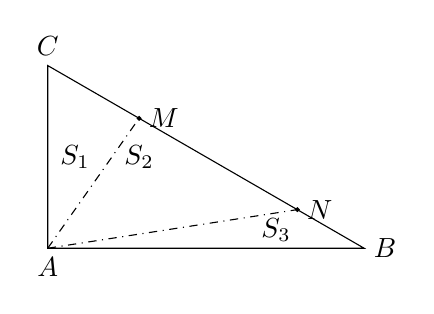
\begin{tikzpicture}[scale=0.33]
		% 计算 sqrt(3) 并存入 \pgfmathresult
		\pgfmathparse{sqrt(3)}
		\coordinate (A)at(0,0);
		\coordinate (B) at(200pt*\pgfmathresult,0);
		\coordinate (C)at(0,200pt);		
		\coordinate (M) at(100pt,200pt-100pt*\pgfmathresult/3);
		\coordinate (N) at($(M)+(100pt*\pgfmathresult,-100pt)$);
		
		% 绘制直角三角形ABC
		\draw (A)--(B)--(C)--cycle;
		\node[below] at(A){$A$};
		\node[right] at(B){$B$};
		\node[above] at(C){$C$};
		\filldraw (M) circle(2pt) node[right]{$M$};
		\filldraw (N) circle(2pt) node[right]{$N$};
		% 标注区域
		\draw[dash dot] (A)--(M);
		\draw[dash dot] (A)--(N);
		
		\node at (30pt,100pt) {$S_1$};
		\node at (100pt,100pt) {$S_2$};
		\node at (250pt,20pt) {$S_3$};
		
	\end{tikzpicture}
\end{center}

（1）当$BN = 200\ \text{m}$时，求木质护栏的长度；

（2）设$\angle NAB = \theta$，请用$\theta$表示水景庭院的面积$S_2$，并求$S_2$的最小值。
\end{question}	
\begin{solution}
	先求出大三角形的基本量：
	\[
	AB=400\sin\dfrac{\pi}{3}=200\sqrt3,
	\qquad
	AC=400\sin\dfrac{\pi}{6}=200.
	\]

	又因为$M,N$都在$BC$上，所以
	\[
	\angle ABN=\angle ABM=\angle ABC=\dfrac{\pi}{6}.
	\]

	（1）

	在$\triangle ABN$中，由正弦定理得
	\[
	\dfrac{BN}{\sin\theta}=\dfrac{AB}{\sin\angle ANB}
	=\dfrac{200\sqrt3}{\sin\left(\pi-\theta-\dfrac{\pi}{6}\right)}
	=\dfrac{200\sqrt3}{\sin\left(\theta+\dfrac{\pi}{6}\right)}.
	\]

	当$BN=200$时，
	\[
	\sin\left(\theta+\dfrac{\pi}{6}\right)=\sqrt3\sin\theta.
	\]
	展开得
	\[
	\dfrac{\sqrt3}{2}\sin\theta+\dfrac12\cos\theta=\sqrt3\sin\theta,
	\]
	所以
	\[
	\cos\theta=\sqrt3\sin\theta,
	\qquad
	\tan\theta=\dfrac{1}{\sqrt3}.
	\]
	于是
	\[
	\theta=\dfrac{\pi}{6}.
	\]

	此时在$\triangle ABN$中，
	\[
	\angle NAB=\angle ABN=\dfrac{\pi}{6},
	\]
	故
	\[
	AN=BN=200.
	\]

	又因为$\angle MAN=\dfrac{\pi}{6}$，所以
	\[
	\angle MAB=\angle MAN+\angle NAB=\dfrac{\pi}{3}.
	\]
	从而在$\triangle ABM$中，
	\[
	\angle AMB=\pi-\dfrac{\pi}{3}-\dfrac{\pi}{6}=\dfrac{\pi}{2},
	\]
	即$\triangle ABM$是直角三角形.

	于是
	\[
	AM=AB\sin\dfrac{\pi}{6}=200\sqrt3\cdot\dfrac12=100\sqrt3,
	\]
	\[
	BM=AB\sin\dfrac{\pi}{3}=200\sqrt3\cdot\dfrac{\sqrt3}{2}=300.
	\]

	而$BN=200$，故
	\[
	MN=BM-BN=300-200=100.
	\]

	所以木质护栏长度为
	\[
	AM+AN+MN=100\sqrt3+200+100=100(3+\sqrt3)\ \text{m}.
	\]

	（2）设$\angle NAB=\theta$.

	由正弦定理，$AN=\dfrac{100\sqrt3}{\sin\left(\theta+\dfrac{\pi}{6}\right)}$，$AM=\dfrac{100\sqrt3}{\sin\left(\dfrac{2\pi}{3}-\theta\right)}$，故
	\[
	S_2=\dfrac12\cdot AM\cdot AN\cdot\sin\dfrac{\pi}{6}=\dfrac{7500}{\sin\left(\theta+\dfrac{\pi}{6}\right)\sin\left(\dfrac{2\pi}{3}-\theta\right)}.
	\]
	令$x=\theta+\dfrac{\pi}{6}$，$y=\dfrac{2\pi}{3}-\theta$，则$x+y=\dfrac{5\pi}{6}$，所以$\sin x\sin y\le \dfrac{1-\cos\frac{5\pi}{6}}{2}=\dfrac{2+\sqrt3}{4}$.
	\[
	\therefore\ S_{2,\min}=\dfrac{7500}{(2+\sqrt3)/4}=30000(2-\sqrt3)\ \text{m}^2,
	\]
	当且仅当$x=y$，即$\theta=\dfrac{\pi}{4}$时取等号.

	\textbf{极限版：}
	\[
	S_2=\dfrac{7500}{\sin\left(\theta+\dfrac{\pi}{6}\right)\sin\left(\dfrac{2\pi}{3}-\theta\right)}.
	\]
	设$x=\theta+\dfrac{\pi}{6}$，$y=\dfrac{2\pi}{3}-\theta$，则$x+y=\dfrac{5\pi}{6}$，故$\sin x\sin y\le \dfrac{1-\cos\frac{5\pi}{6}}{2}=\dfrac{2+\sqrt3}{4}$.
	\[
	\therefore\ S_{2,\min}=30000(2-\sqrt3)\ \text{m}^2,
	\qquad \theta=\dfrac{\pi}{4}.
	\]
\end{solution}


\end{document}